\documentclass{article}

\usepackage[a4paper,margin=1.15in,footskip=0.25in]{geometry}

\usepackage[utf8]{inputenc}
\usepackage[english]{babel}
\usepackage{textpos}
\usepackage{textcomp}
\usepackage{amsmath}
\usepackage{amssymb}
\usepackage{amsfonts}
\usepackage{graphicx}
\usepackage{epstopdf}
\usepackage{algorithmic}
\usepackage{verbatim}
\usepackage{textcomp}
\usepackage{varwidth}
\usepackage[linesnumbered,ruled]{algorithm2e}

% For displaying code
\usepackage{listings}

% Theorem
\newtheorem{theorem}{Theorem}

% lists
\usepackage{outlines}
\usepackage{enumitem}
\newenvironment{tight_enum}{
\begin{enumerate}[label=\alph*.]
\setlength{\itemsep}{0pt}
\setlength{\parskip}{0pt}
}{\end{enumerate}}

% \subsubsubsection{}
\setcounter{secnumdepth}{5}
\setcounter{tocdepth}{5}
\newcommand\simpleparagraph[1]{%
  \stepcounter{paragraph}\paragraph*{\theparagraph\quad{}#1}}

\usepackage{listings}
\usepackage{color}
\usepackage{xcolor}
\usepackage{mdframed}

\definecolor{dkgreen}{rgb}{0,0.6,0}
\definecolor{gray}{rgb}{0.5,0.5,0.5}
\definecolor{mauve}{rgb}{0.58,0,0.82}

% \usepackage{courier}
\lstset{%frame=tb,
language=C++,
aboveskip=3mm,
belowskip=3mm,
showstringspaces=false,
columns=flexible,
basicstyle={\small\ttfamily},
numbers=none,
numberstyle=\tiny\color{gray},
keywordstyle=\color{blue},
commentstyle=\color{dkgreen},
stringstyle=\color{mauve},
breaklines=true,
breakatwhitespace=true,
tabsize=3
}

%%%%%%%%% BEGIN DOCUMENT %%%%%%%%%
%%%%%%%%% BEGIN DOCUMENT %%%%%%%%%
%%%%%%%%% BEGIN DOCUMENT %%%%%%%%%

%% Used tt when referring to function

\begin{document}

\title{Parallel Orthogonal Recursive Bisection}
\author{Team Metropolis: \\
		Jamshid 'James' Farzidayeri, JJ Lay, and Graham West}
\date{COMS 7900, Capstone}

\maketitle

\begin{abstract}
In our first project, we implemented a parallel sorting algorithm which utilized a local gradient-type optimization search to equalize the amount of data across different compute nodes in order to achieve maximum efficiency. In this project, we applied this algorithm to the problem of parallel orthogonal recursive bisection (ORB), i.e., the construction of $k$-d trees. In order to do this, we had to heavily modify the sorting algorithm in several ways, including 1) turning it into a callable function, 2) letting the rank 0 head node perform work while still managing the tasks, 3) incorporating the use of different MPI communicators, and 4) altering the adaptive binning technique for better convergence.

In this paper, we will discuss how our $k$-d tree algorithm works, how we solved the various issues plaguing parallel sort (mentioned above), and how we tested and validated our work. We conclude with a discussion of the major difficulties in completing this project and how these difficulties could be minimized in the future.
\end{abstract}


\tableofcontents


%%%%%%%%%%%%%
%%% NEW SECTION %%%
%%%%%%%%%%%%%
\section{Introduction}

% GW
STATEMENT OF THE PROBLEM: talk about orthogonal recursive bisection ORB, needed to search all the data with 3 radii and 501 file centers, return table of counts


% farzi
\subsection{Workflow}
One of the major issues we encountered during our last project was overwriting each other’s GitHub submissions. Our resolution was to create a master branch and three sub branches. Each person was assigned a sub branch that they could modify as they pleased. However, a modification in the master branch parallel approved folder required two or more party members consent. This vastly reduced the amount of issues encountered during push/pull request. 
Another adjustment we made for our development process was to write our code together and in an accommodating space as opposed to assigning individual sections of code. We met on a regular basis, generally starting during our scheduled class period and extending through the lunch period. This allowed us to catch errors quickly, avoid merge conflicts and most significantly improved everyone's knowledge of how each component of the code works. 
When the project was assigned each team member prototypes a version of serial KD tree in their preferred language. After several meetings it was determined that Graham’s MatLab implementation would be used as the guide for the project. 

\subsection{Variables and conventions}
%%% NOTE %%%
%%% NOTE %%%
% 1) be consistent with the indices:
% 2) say head node (not master node)
% 3) say worker (not node) whenever possible
%%% NOTE %%%
%%% NOTE %%%

\begin{mdframed}[backgroundcolor=blue!20]
	Counts:
	\setlength\itemsep{0.1pt}
	\setlength\parskip{0.1pt}
	\begin{itemize}
		\setlength\itemsep{0.1pt}
		\setlength\parskip{0.1pt}
		\item $N$: number of nodes
		\item $M$: max number of allowed time steps
		\item $L$: number of lines to read per file
		\item $L_w$: number of lines on the $w$th worker
		\item $D$: total number of lines/data points
	\end{itemize}
\end{mdframed}

\begin{mdframed}[backgroundcolor=blue!20]
	Indices:
	\setlength\itemsep{0.1pt}
	\setlength\parskip{0.1pt}
	\begin{itemize}
		\setlength\itemsep{0.1pt}
		\setlength\parskip{0.1pt}
		\item $m = 0, \cdots, M$ is the time step of the bin adaptation scheme (likely less than $M$)
		\item $n = 0, \cdots, W$ spans the nodes
		\item $i = 0, \cdots, N$ spans the bin edges/indices
		\item $j = 0, \cdots, N-1$ spans the bin counts (this will occasionally subscript binI/E as well)
		\item $\ell_w = 0, \cdots, L_n-1$ spans the lines on the $n$-th node
		\item $k = 0, \cdots, 3$ is the data column being sorted
	\end{itemize}
\end{mdframed}

\begin{mdframed}[backgroundcolor=blue!20]
	Variables:
	\setlength\itemsep{0.1pt}
	\setlength\parskip{0.1pt}
	\begin{itemize}
		\setlength\itemsep{0.1pt}
		\setlength\parskip{0.1pt}
		\item $\textrm{data}^n_{4\ell+k}$: data point on $\ell$th line and $k$th column on the $n$-th node
		\item ${E}^m_j$: bin edges (0 indexed) at time step $m$
		\item ${I}^{n,m}_j$: bin indices on node $n$
		\item ${C}^{n,m}_j$: bin counts on node $n$ at time step $m$
		\item ${C}^m_j$: total bin counts on head node (sum of node C's) at time step $m$
	\end{itemize}
\end{mdframed}


%%%%%%%%%
%
% Section: Implementation
%
%%%%%%%%%

\section{Implementation}
% JJ

Here we discuss our implementation of the code

we used C++ with C MPI calls, mpirun, qsub/qlogin, valgrind

\subsection{\texttt{main}}
% GW
import: gets the list of files and imports their data into an array


build: we build the tree using ORB to partition the data


search: import the 501-st data file and perform a search on each, summing the total number of points found over several radii


%%%%%%%%%
%
% Subsection: K-d Tree
%
%%%%%%%%%

\subsection{K-d tree}
%
% JJ, talk about the Tree struct and what all fields it has
%

The design of the k-d tree required storing information for organizing the parallel distribution of the data and the data held locally on the node. Rather than create two different type of structures, the code utilized a single C \texttt{struct} which is defined as:

\lstset{language=C++, keepspaces=true}
\begin{lstlisting}
struct Tree {
    // Pointers used for local tree
	Tree *p;    // Parent
	Tree *l;    // Left child
	Tree *r;    // Right child
	int i;      // Sort dimension used to split this node
	int source; // Which buildTree function created it

    // Pointers used for parallel tree
	MPI_Comm parentComm;  // Parent communicator
	MPI_Comm leftComm;    // Left child communicator
	MPI_Comm rightComm;   // Right child communicator
	MPI_Comm thisComm;    // Communicator that the node belongs to

    // Each node in the tree has a unique identifier
	string name;

    // For nodes with children, this holds the min and max for
    // the child nodes
	double x1;  // Min x
	double x2;  // Max x
	double y1;  // Min y
	double y2;  // Max y
	double z1;  // Min z
	double z2;  // Max z

	int depth;  // Depth of the node in the tree
	int n;      // Number of points

	double c[4];    // Center of this tree
	double radius;  // Radius of this tree

	double d[4];   // Data point coordinates
	double index;  // File row index from source data
}
\end{lstlisting}

%%%%%%%%%
%
% Subsubsection: Constants
%
%%%%%%%%%

\subsubsection{Constants}

C preprocessor identifiers were defined and used in place of numeric constants for readability. Data points were defined as an array of \texttt{double} of size four consistently even when only three values were needed. The four positions were referenced using:

\lstset{language=C++, keepspaces=true}
\begin{lstlisting}
#define _INDEX_   0  // Row index from source datafile
#define _X_       1
#define _Y_       2
#define _Z_       3
\end{lstlisting}

A single tree is create and populated by both the parallel and serial versions of \texttt{buildTree}. To aid with debugging, each node is marked with an identifier to show which function created it. The identifiers for the sources are:

\lstset{language=C++, keepspaces=true}
\begin{lstlisting}
#define _Source_buildTree_unknown     0
#define _Source_buildTree_parallel   -1
#define _Source_buildTree_serial     -2
\end{lstlisting}



%%%%%%%%%
%
% Subsubsection: Parallel Variable
%
%%%%%%%%%

\subsubsection{Parallel variables}

The \texttt{struct} variables used during the initial division of the tree among the nodes and their purpose are:

\begin{description}
    \item[\texttt{i}]{The dimension that was split by the MPI communicator.}
    \item[\texttt{source}]{During the parallel phase, this value is set to \texttt{\_Source\_buildTree\_parallel}.}
    \item[\texttt{parentComm}]{The parent MPI communicator that created this node. The root node stores a value of \texttt{MPI\_COMM\_SELF} in lieu of a null.}
    \item[\texttt{leftComm}]{}
    \item[\texttt{rightComm}]{}
    \item[\texttt{thisComm}]{}
\end{description}

\lstset{language=C++, keepspaces=true}
\begin{lstlisting}
	int i;      // Sort dimension used to split this node
	int source; // Which buildTree function created it

    // Pointers used for parallel tree
	MPI_Comm parentComm;  // Parent MPI communicator
	MPI_Comm leftComm;    // Left child MPI communicator
	MPI_Comm rightComm;   // Right child MPI communicator
	MPI_Comm thisComm;    // MPI communicator that the node belongs to

    // Each node in the tree has a unique identifier
	string name;

    // For nodes with children, this holds the min and max for
    // the child nodes
	double x1;  // Min x
	double x2;  // Max x
	double y1;  // Min y
	double y2;  // Max y
	double z1;  // Min z
	double z2;  // Max z

	int depth;  // Depth of the node in the tree
	int n;      // Number of points

	double c[4];    // Center of this tree
	double radius;  // Radius of this tree
\end{lstlisting}

\begin{figure}
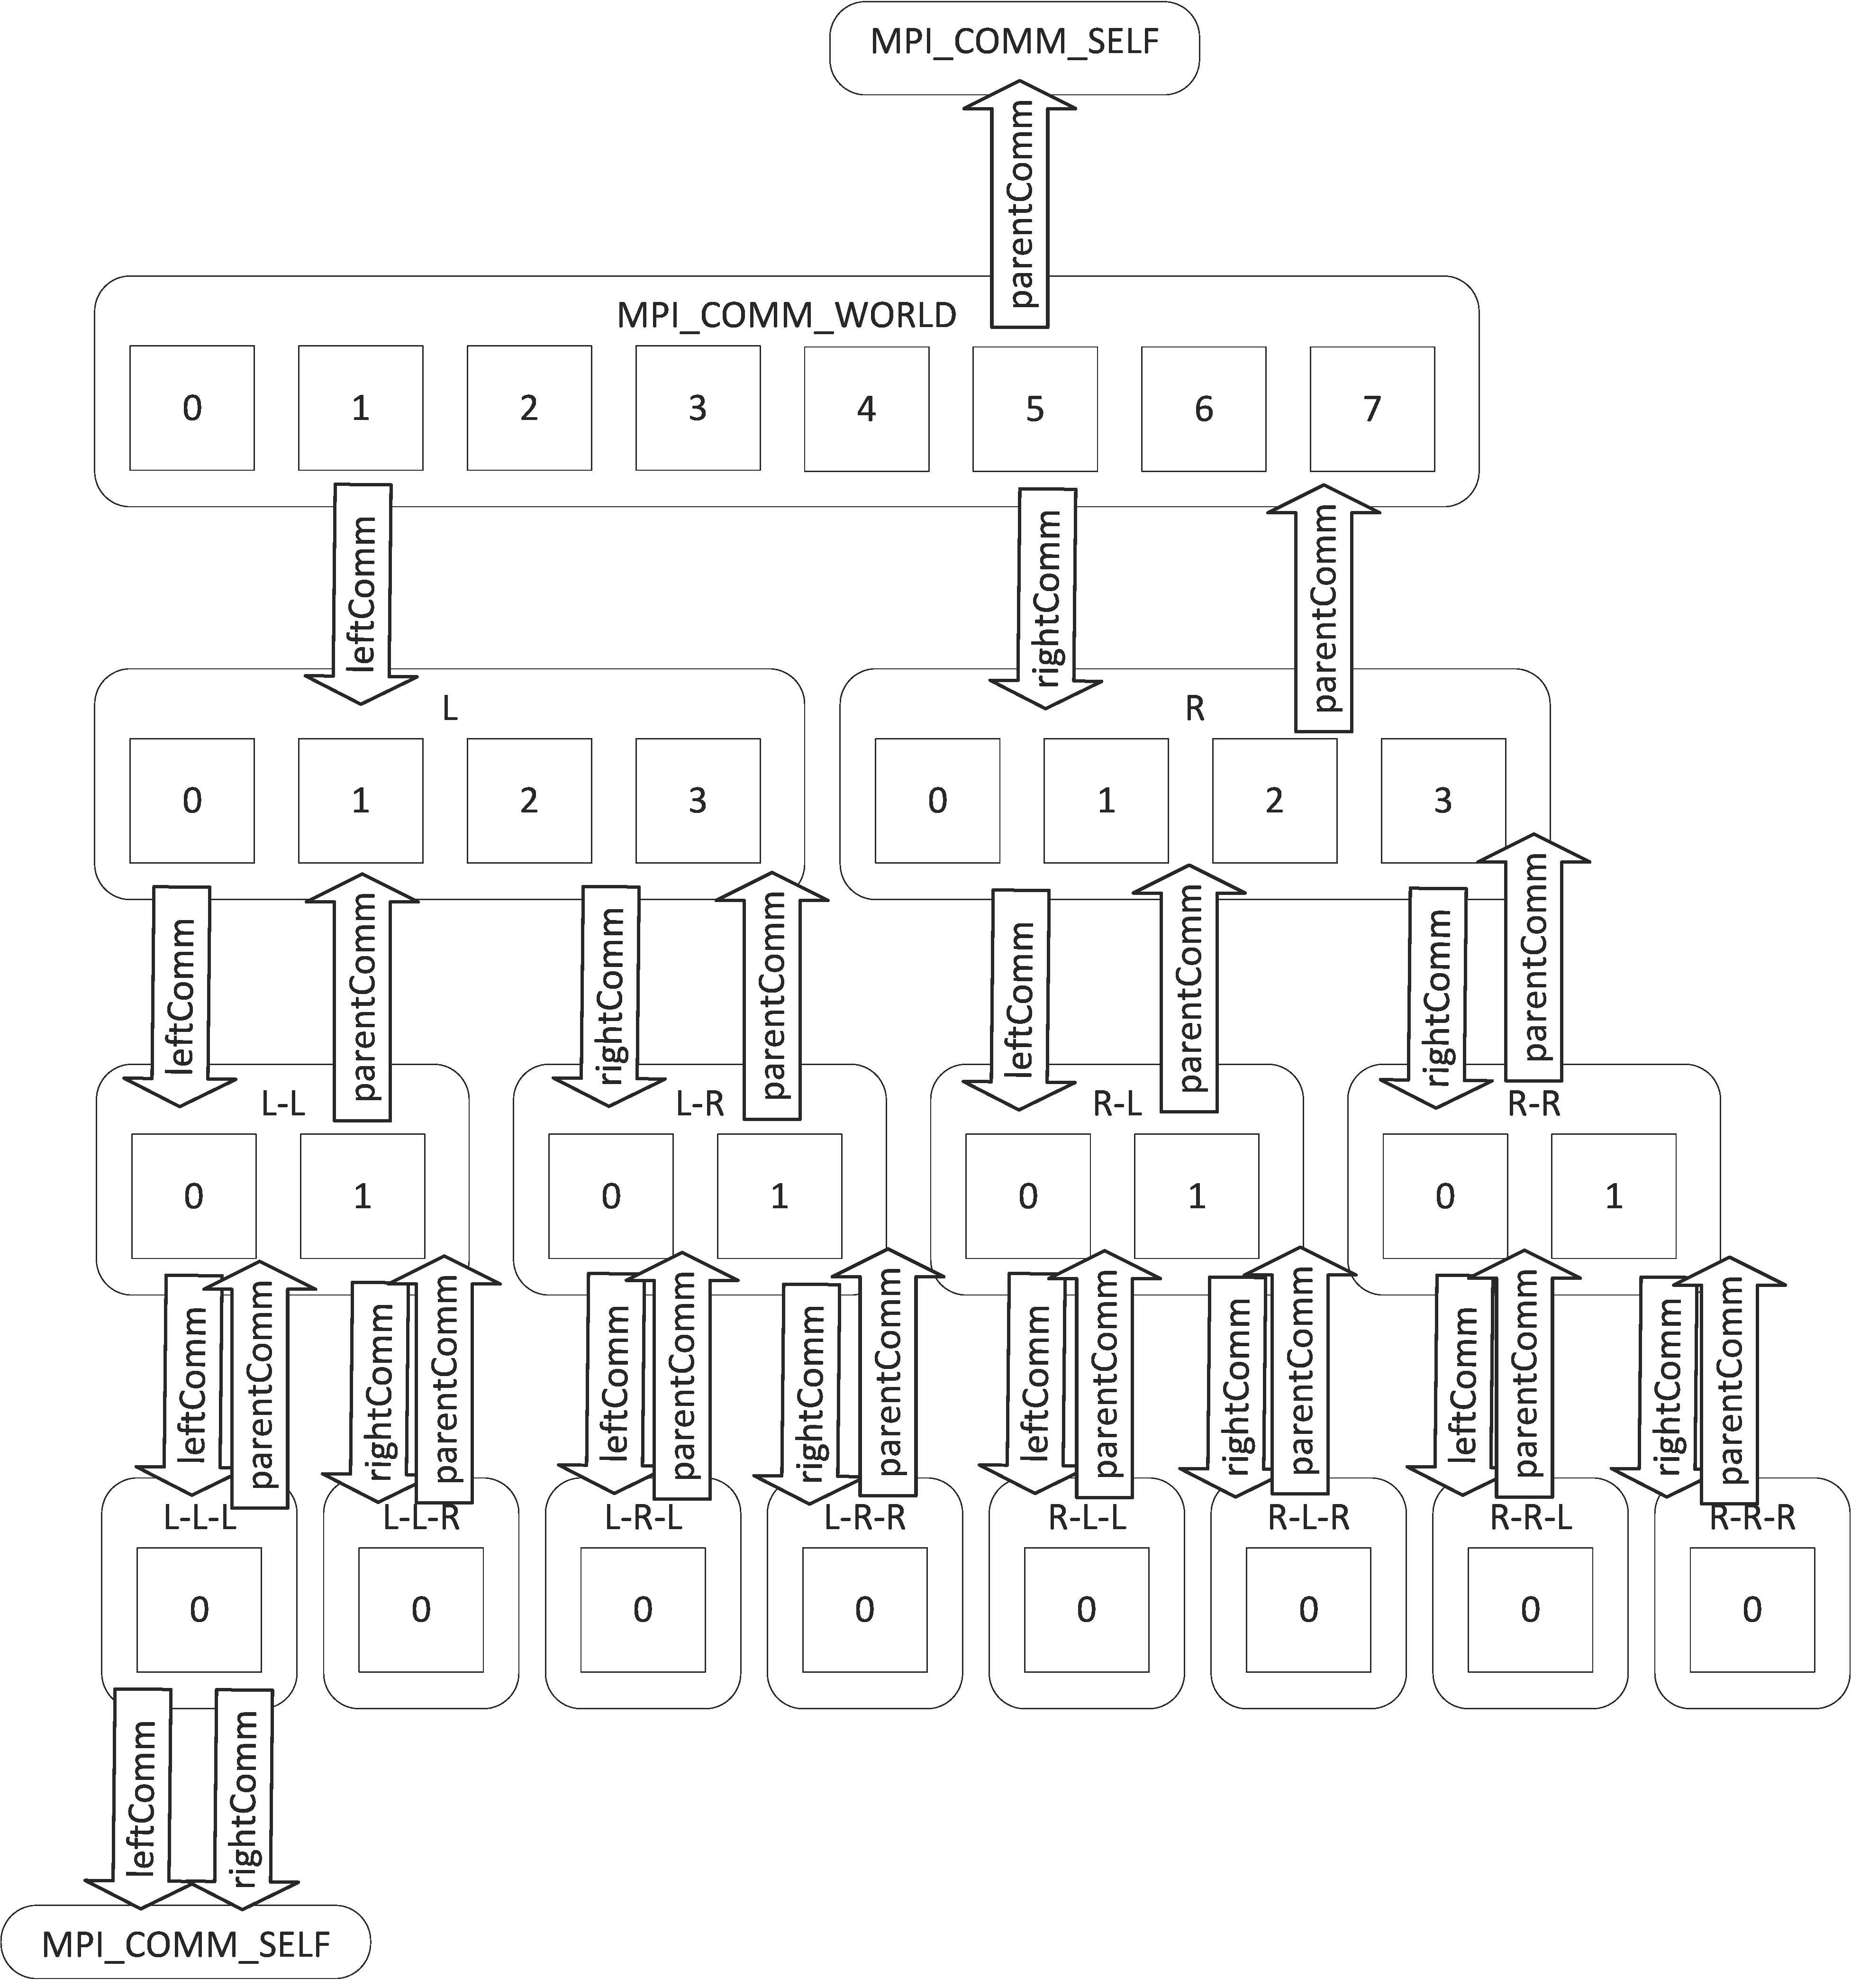
\includegraphics[width=0.9\textwidth]{images/communicators.png}
\caption{Example of parallel variables using eight nodes}
\end{figure}
%%%%%%%%%
%
% Subsubsection: Serial variables
%
%%%%%%%%%

\subsubsection{Serial variables}

\lstset{language=C++, keepspaces=true}
\begin{lstlisting}
    // Pointers used for local tree
	Tree *p;    // Parent
	Tree *l;    // Left child
	Tree *r;    // Right child
	int i;      // Sort dimension used to split this node
	int source; // Which buildTree function created it

    // Each node in the tree has a unique identifier
	string name;

    // For nodes with children, this holds the min and max for
    // the child nodes
	double x1;  // Min x
	double x2;  // Max x
	double y1;  // Min y
	double y2;  // Max y
	double z1;  // Min z
	double z2;  // Max z

	int depth;  // Depth of the node in the tree
	int n;      // Number of points

	double c[4];    // Center of this tree
	double radius;  // Radius of this tree
\end{lstlisting}

%%%%%%%%%
%
% Subsubsection: Data point variables
%
%%%%%%%%%

\subsubsection{Data point variables}

\lstset{language=C++, keepspaces=true}
\begin{lstlisting}

    // Pointers used for local tree
	Tree *p;    // Parent
	Tree *l;    // Left child
	Tree *r;    // Right child

	int source; // Which buildTree function created it

    // Each node in the tree has a unique identifier
	string name;

	int depth;  // Depth of the node in the tree
	int n;      // Number of points

	double d[4];   // Data point coordinates
	double index;  // File row index from source data
}
\end{lstlisting}


%%%%%%%%%
%
% Subsection: Building the tree
%
%%%%%%%%%

\subsubsection{Building the tree}
% General notes on the method...

\paragraph{\texttt{buildTree}}
% farzi, just add the listing
This function gets the number of compute nodes $q$ available in the current communicator and determines which function to run. If $q>1$, then we can still do a parallel sort with 2 compute nodes, so \texttt{buildTree\_parallel} is entered. If $q=1$, then \texttt{buildTree\_serial} is entered.


\paragraph{\texttt{buildTree\_serial}}
This was the first function written after our initial prototyping phase was completed. It essentially performs a serial version of ORB which can be executed on a single compute node.

%
% JJ, you wanna write this since you wrote the program?
%

Upon completion, \texttt{buildTree\_serial} calls itself instead of \texttt{buildTree} since we still have $q=1$.


\paragraph{\texttt{buildTree\_parallel}}
This function performs essentially the same tasks as \texttt{buildTree\_serial}, but utilizing multiple nodes for speedup. Specifically, it takes advantage of \texttt{parallelSort} in order to speed up the partitioning of the data along the longest axis (determine by \texttt{getSortDim}, discussed below). After the data has been sorted, the data is split by placing lower half (w.r.t. the sorted data values) of the compute nodes into a left communicator and the upper half into a right communicator. Each half then calls \texttt{buildTree}.

% Upon completion, \texttt{buildTree\_parallel} has spawned 2 new communicators (a left and a right) each of which has half as many compute nodes as the parent communicator. All of the nodes from each side then call \texttt{buildTree} so that they can perform the $q$ check.


\paragraph{\texttt{getSortDim}}
This function is used by \texttt{buildTree\_parallel} in order to determine which is the longest axis, i.e., the sort dimension. In addition to this, it also fills in the struct for the current tree node with the global min/max in all three dimensions. To do this, each node gets its own min/max for each axis and sends them to rank 0 (w.r.t. the current communicator). Rank 0 then determines the global min/max and them MPI\_Bcast's those values back to the other ranks. This allows each communicator to sort their data independently along different axes. The center of the bounding box defined by these values min's/max's is also stored in the tree struct. 


\subsubsection{Searching the tree}



\paragraph{\texttt{searchTree\_serial}}
% GW
This function is called by all ranks and returns an integer which equals the number of points found by the rank that called it. It takes as arguments the point and radius (which specifies a search sphere) and the root of the tree created by \texttt{buildTree}. To perform the search, a check is done to determine of the search sphere intersects the bounding sphere of each data partition:
\begin{equation}
		test
\end{equation}
If this check returns false, then there are no data points within the search sphere contained in that partition. If true, then another check is performed to check if the partition contains only a single point (if so, it increments the found count); otherwise the search branches and calls itself, creating a recursive loop.


ADD PSEUDOCODE


\paragraph{\texttt{search501}}
%
% JJ, edit if you wan since you wrote most of this
%

Each node calls this function which reads the 501-st data file, whose contents are the centers of the search spheres. It then loops through \texttt{searchTree\_serial} through all of the sphere centers for three different radii (0., 0., 0.). The counts on each node are then stored. After all searches are complete, then an MPI\_Reduce is performed by all nodes, thus adding all of the counts into a single array which is exported to a file.


\subsection{Altered parallel sorting}
We had to adjust our parallel sorting algorithm a great extend to integrate it into the new project.


\subsubsection{\texttt{parallelSort}}

% GW, farzi

\paragraph{Conversion to function}
One of our first obstacles was modifying our original parallelSort program to work for this project. The first issue was having parallelSort operate as a function. We accomplished this by removing the MPI setup and Data Import sections from parallelSort and placing them into a new Main. While doing this we encountered issues with how the data was passed using both a pointer and array notation. Because several functions within the parallelSort function would need to change both the number of rows and the data we had to pass as pointers and pointers to arrays. 


\paragraph{Making rank 0 do work}
The second issue was our use of rank 0 as the manager in our original parallelSort program. Our implantation of parallelSort had rank 0 manage while all the other ranks contained and performed operations on the actual data. However, when utilizing a KD tree all of the ranks are needed otherwise each time the tree forked and a new communication branch was formed the process would lose a rank due to a new rank 0 being formed. To resolve this problem  we had to make several clever adjustments in the sections of the code, most notably the adapt binning section. Other sections just needed to have the iteration increment from 0 instead of 1. 
\paragraph{Using different communicators}
Since kdtree requires multiple comms, it was necessary that parallel sort (any many functions it contains) was given the current communicator. This was not a terribly difficult modification, but it was quite tedious since there were many functions which required alterations to their header files.


\subsubsection{\texttt{adaptBins}}
Although our original adaptive binning scheme performed well, we wanted something which could do even better since $k$-d trees require many parallelSort calls. As a review, here is our original method:
\begin{equation}
	\begin{split}
		\Delta C & = 2.0 ( C^{m}_{i+1} - C^{m}_i ) / ( C^{m}_{i+1} + C^{m}_i ) \\
		\Delta E & = E^m_{i+1} - E^m_i \\
		E^{m+1}_i & = E^m_i + \alpha \Delta C \Delta E
	\end{split}
\end{equation}
% added scale factor
where $C$ are the bin counts, $E$ are the bin edges, and $\alpha < 0.5$. This method will occasionally devolve into oscillatory behavior and not converge to the correct value. To combat this in the $k$-d tree project, we added a scale factor $S$ which decreases over time:
\begin{equation}
	\begin{split}
		S & = 1 - (1 - 0.1) (1 - \textrm{exp}(-0.03 m) \\
		E^{m+1}_i & = E^m_i + \alpha S \Delta C \Delta E
	\end{split}
\end{equation}

Since this method is local, it converges slowly at bin edges far away from high-density clusters. As such, we attempted to replace this method with a global method which uses linear interpolation to estimate where the bins would be evenly distributed. Define the function $\hat C(x)$ as the linear approximation of the cumulative count distribution of the data points (so that it normalizes to the number of data points, not unity). Then,
\begin{equation}
		\hat C(x) = \hat C(E^m_{i'}) + C^m_{i'} \dfrac{x - E^m_{i'}}{E^m_{{i'}+1} - E^m_{i'}} = (i+1) \dfrac{D}{N}
\end{equation}
where $i'$ is the maximum index such that $\hat C(E_{i'}) < (i+1) \dfrac{D}{N}$ (note that $i'$ and $i$ are distinct integers). The right equality implies that we should solve for the value of $x$ such that it holds. This $x$ value will be the new $i$-th bin edge, $E^{m+1}_i$. Therefore,
\begin{equation}
		E^{m+1}_i = E^m_{i'} + \bigg( (i+1) \dfrac{D}{N} - C(E^m_{i'}) \bigg) (E^m_{{i'}+1} - E^m_{i'}) / C^m_{i'}
\end{equation}

We discovered that this adaptation technique performs very will in initial steps of adaptation, but is prone to oscillations near clusters of points. Now, since each of the two methods perform better and worse in different contexts, are solution was to simply alternate between at each step. This solved all of our convergence issues in testing. (Note that we still use the same binary search-based binning technique and stopping criterion from the previous project.)





%%%%%%%%%%%%%
%%% NEW SECTION %%%
%%%%%%%%%%%%%
\section{Validation}


% GW, farzi
\subsection{Two MATLAB demos}
Should these not be in the paper since animation is a pain without adobe??? Leave it for the presentation where we can just run it?

\subsubsection{2D animation of tree building}


\subsubsection{3D tree partitions from different orientations}
In addition to our use of MATLAB for prototyping, we also used it to validate our tree building algorithm.


\subsection{Other}
able to get same counts for different number of nodes




%%%%%%%%%
%
% Section: Results
%
%%%%%%%%%

\section{Results}

% JJ

%%%%%%%%%
%
% Subsection: Timing Testing
%
%%%%%%%%%

\subsection{Timing Testing}


%%%%%%%%%
%
% Subsection: Search Results
%
%%%%%%%%%

\subsection{Search Results}



%%%%%%%%%%%%%
%%% NEW SECTION %%%
%%%%%%%%%%%%%
\section{Conclusion}

% everyone

\subsection{Challenges}



\subsection{Future Work}



%%%%%%%%%%%%%
%%% NEW SECTION %%%
%%%%%%%%%%%%%
\section{Bibliography}

\end{document}
